\documentclass{article}
\usepackage[utf8]{inputenc}
\usepackage{graphicx}
\usepackage{subfig}
\usepackage{amsmath}

\title{Digital Logic Design Assignment 10 - EC2011-19}
\author{S . Manasa}

\begin{document}

\maketitle

\section{Question}
When the output Y in the circuit below is '1',it implies that the data has
\begin{center}
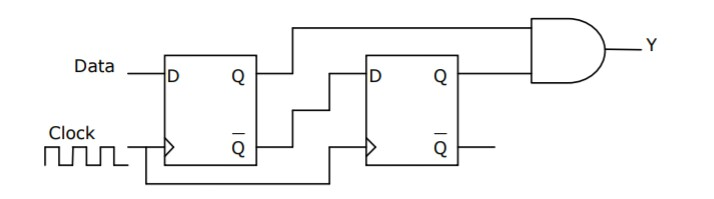
\includegraphics[width=300,height=100]{Figure.jpeg}
\end{center}
\\
(A) changed from 0 to 1\\
(B) changed from 1 to 0\\
(C) changed in either direction\\
(D) not changed\\


\section{Solution}
In this problem there are two D-flip flops and one and gate.
The output of and gate is Y which is the output of the above sequential circuit.\\ For our convenience let us take the first flip flop as A flip flop and second flip flop as B flip flop.\\~


For $A$ flip flop
\begin{itemize}
    \item Input is $D_A$
    \item Outputs are $Q_A$ and $\overline{Q_A}$
\end{itemize}
\\~

For $B$ flip flop
\begin{itemize}
    \item Input is $D_B$
    \item Outputs are $Q_B$ and $\overline{Q_B}$
\end{itemize}
 \\~
 
 Now we need to find out the change in data when output Y is equal to 1.

 From the figure , it is clear that
 \begin{equation}
     Q_A = D_A = Data 
\end{equation}

 \begin{equation}
    Q_B = D_B = \overline{Q_A}
\end{equation}

\begin{equation}
     Y = Q_A.Q_B
\end{equation}
 \subsection{State transition Diagram}
 \begin{center}
    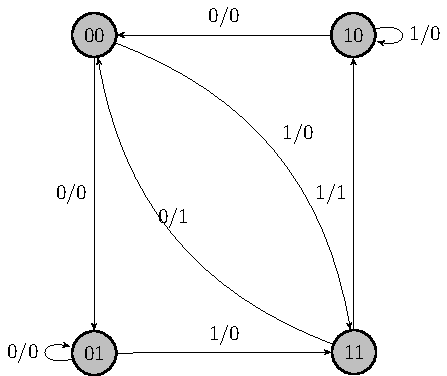
\includegraphics[width=300,height=150]{State_diagram.pdf}
\end{center}

\subsection{State transition Table}
\begin{center}
    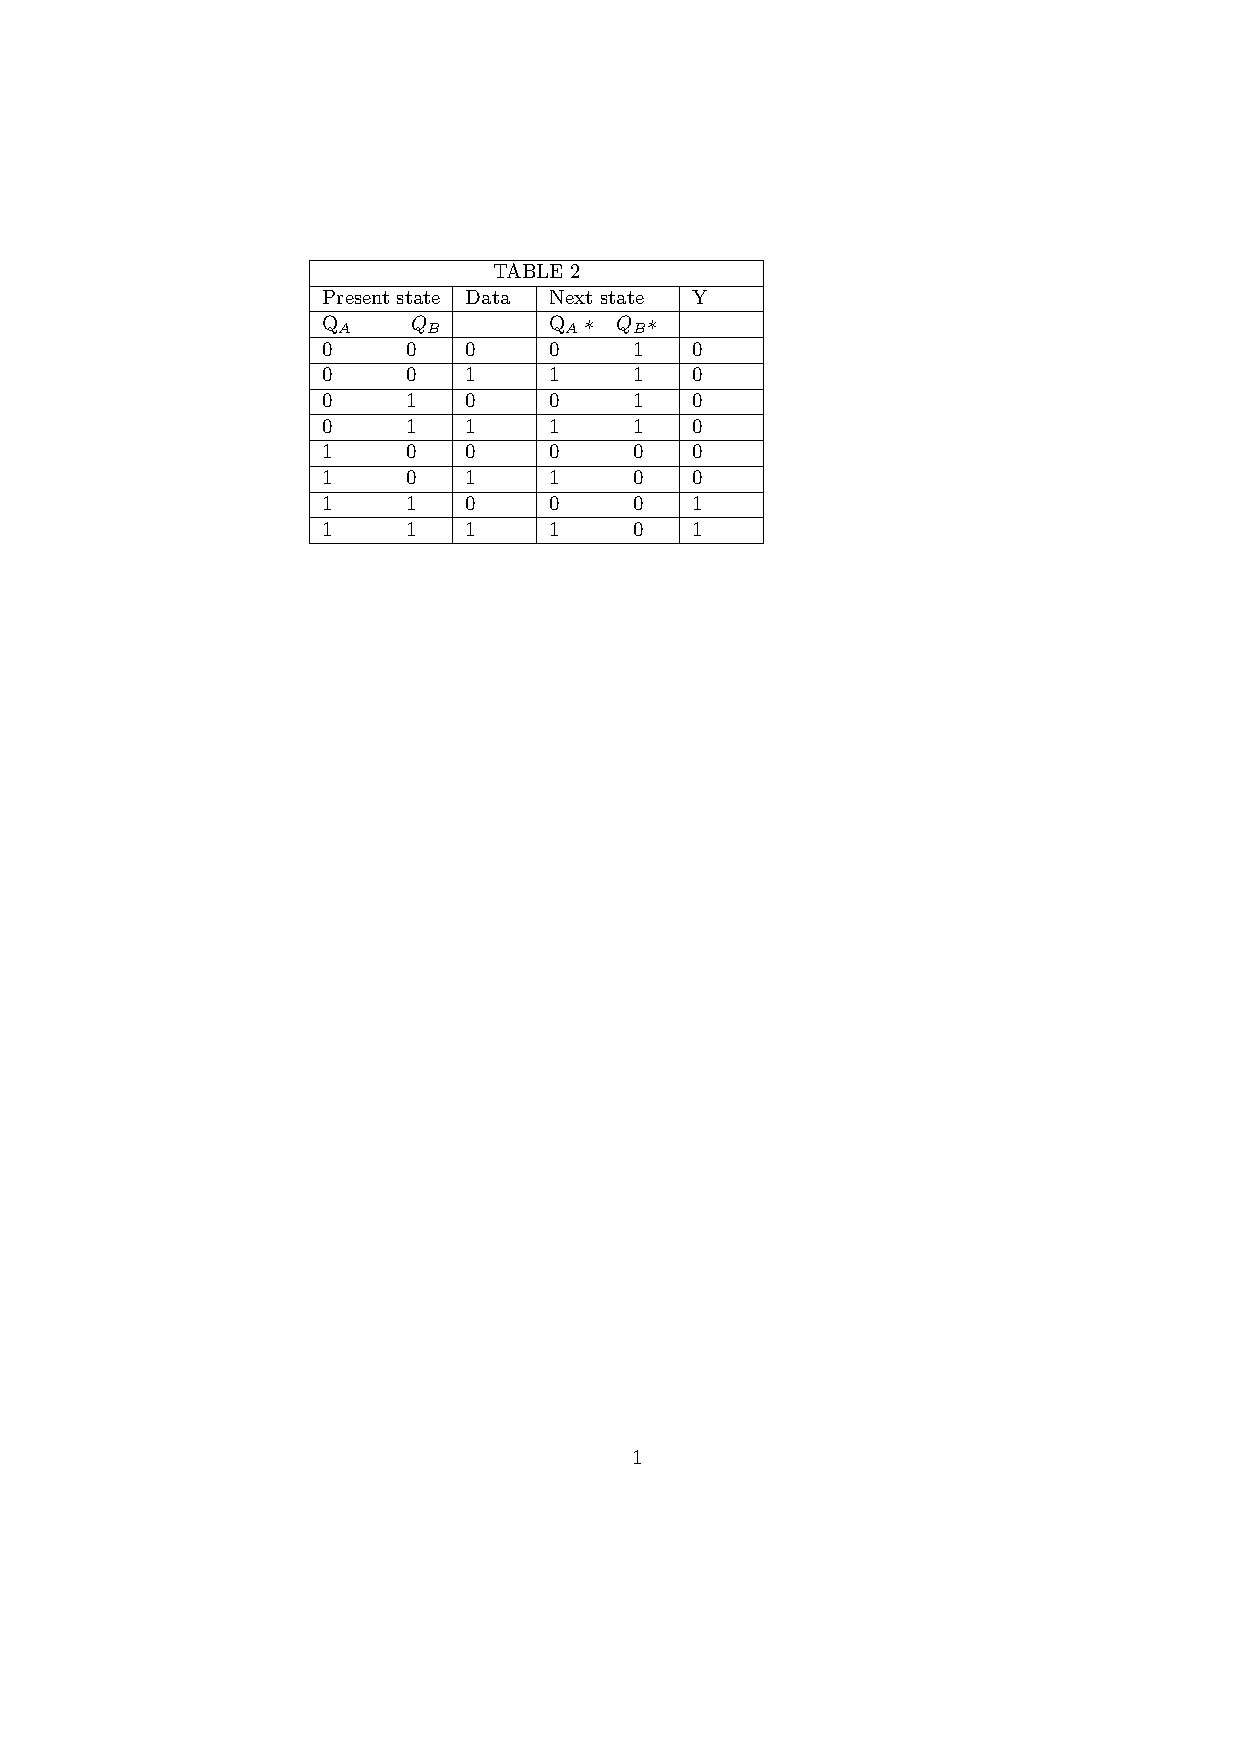
\includegraphics[width=600,height=900]{State_transition_table_c_code.pdf}
\end{center}
\subsection{Table} 

    \begin{table}
    \centering
    \begin{tabular}{|c|c|c|c|}
    \hline
    Clock & Data & $Q_A$ & $Q_B$ \\
    \hline
    \hline
    - &  & 0 & 0 \\
    \hline
    1st Pulse & $D_1$ & $D_1$ & 1\\
    \hline
    2nd Pulse & $D_2$ & $D_2$ & $\overline{D_1}\\
    \hline
 
    \end{tabular}
    \end{table}
\begin{itemize}
    \item When the clock is not given to the flip flops then $Q_A$ and $Q_B$ will remain in their reset state
    \item For the first clock pulse , we give the data as $D_1$
    \begin{itemize}
        \item From equation (1) we get $Q_A = Data$. Since data = $D_1$,$Q_A$ = $D_1$ \\~
         \item From equation (2) we get $Q_B = \overline{Q_A}$. Since $Q_A$ = 0,$Q_B$ = 1
        \end{itemize}
    \item  For the second clock pulse , we give the data as $D_2$
    \begin{itemize}
        \item From equation (1) we get $Q_A = Data$. Since data = $D_2$,$Q_A$ = $D_2$ \\~
         \item From equation (2) we get $Q_B = \overline{Q_A}$. Since $Q_A$ = $D_1$,$Q_B$ = $\overline{D_1}$
        \end{itemize}   
\end{itemize}
\subsection{Answer}

Now we will generalise the case
\begin{itemize}
    \item The output of first flip flop $Q_A$ is equal to $present \hspace{2} data$
    \item The output of second flip flop $Q_B$ is equal to compliment of $previous \hspace{2} data$
\end{itemize}
We know that $Y = Q_A.Q_B$ \\~

This means $Y=(present data).(\overline{previous data})$ \\~

So the output of Y is equal to 1 only when the present data is equal to 0.So the data must change from 0 to 1.
\\~

In this way option (A) is the correct answer
    



\end{document}